\setcounter{secnumdepth}{4}
\section{Neural Networks}  \label{cha:foundations_basics_nn}
This section is organized as follows. In this section first providing a brief history of deep learning ...
\subsection{The Beginnings of Artificial Neural Networks}
%if you like to extend you can add country and the field of the people
Alan Turing who is considered to be the father of computer science laid  the first foundations of artificial intelligence with his paper titled \textit{"Computing machinery and intelligence"} in 1950s. In his paper he introduced the Turing test....   

The second founding event of artificial intelligence was a \textit{Dartmouth Summer Research Project on Artificial Intelligence}, 1956 Workshop. The Workshop lasted six to eight weeks as brainstorming sessions where McCarthy coined the term "artificial intelligence" in 1955.


Neural network history begins, with the seminal paper by Walter Pitts and Warren McCulloch titled A Logical Calculus of Ideas Immanent in Nervous Activity. The paper describes the idea of the artificial neural networks with relevant definitions which we still rely on them today. Another hero of deep learning is Frank Rosenblatt an American psychologist. F. Rosenblatt discovered the \textit{perceptron learning rule} which explains how to update the parameters (weights) of a neural network. Besides his discovery of perseptron,  Rosenblatt also put forward an idea of multilayered networks that are similar to convolutions neural networks today. This can be considered to start of the journey towards \textit{deep learning}. Despite of the developments in artificial neural networks,  the book written by Marvin Minsky and Seymour Papert in 1969 caused huge setback. In the book, Minsky and Papert tried to prove that perceptrons are simple linear classifier and has major computational limitations such as XOR function. Further, the book had great impact on discorement of further deveopment of artifical neural networks. Thereafter, another development which enabled the community to train a neural network with more than one layer, was the discovery of Backpropagation by Rumelhart, Hinton and Williams. 

In early 1990s, some people from AI community shifted towards support vector machines (SVM) due to its performance and simplicity. SVMs mainly developed by psychologists and cognitive scientists. However, two major events occurred in the late 1990s, (1) the invention of The long short-term memory by Hochreiter and Schmidhuber in 1997; (2) in 1998 LeCun, Bottou, Bengio and Haffner produced the first convolutional neural network called LeNet-5. Finally, in 2006 Hinton, Osindero and Teh published a paper which introduces deep belief networks (DMB). After this paper a new period of AI began.
\subsection{The Basic Architecture of Neural Networks} 
%book:Neural Networks and Deep Learning, Charu C. Aggarwal
In this section basic architecture of single-layer and multi-layer neural networks have been discussed. Single-layer neural networks are also refered as \textit{perceptrons} which have a output layer and the set of inputs are directly mapped to the output layer%you can say only a node. 
. Moreover, multi-layer neural networks which do not have only input and output layers but also hidden layers. This type of neural networks are also known as \textit{feed-forward networks}. 
%This chapter aims for providing an overview on the
\subsubsection{Single-layer Neural Networks: Perceptron}
Perceptron is the simplest neural network architecture contains an input layer and output layer which is only a single node. Fig illustrates a simple perceptron architecture with and without bias neuron. The input layer simply transmits the each individual feature to the output layer by multiplying them with the corresponding weight (e.g., $x_1$ would be multiplied with $w_1$). Note that since the input layer does not perform any computation, often it is not included in the count of the number of layers in a neural network.

Given a training set where each instance is of a form ($\overline{X}$, $y$) where $\overline{X}=[x_1,x_2,...,x_d]$ denote an input variable with \textit{d}-dimensional features, $b$ is bias and $y$ is an output that $y \in{\{-1, +1\}}$. Let $\overline{W}=[w_1,w_2,...,w_d]$ denote the weight of the edges and the output $\hat{y}$ is computed as follows: 
%Formula 1.2

The sign function maps a real value to either \num{+1} or \num{-1} as $y \in{\{-1, +1\}}$. In other words, the sign function here serves the role of an \textit{activation function}. Depending on the application at hand different type of activation functions such as \textit{logistic regression classifier} can be utilized. The depicted scenario appropriate for binary classification task where the output of the sign function, i.e., \num{-1} or \num{+1} corresponds to a class label. 


The optimization of the perceptron algorithm is performed heuristically and the goal of the algorithm is to minimize the following heuristically motivated loss function with respect to all training instances:

The weights then updated based on the error value as follows:
%Formula 1.3
where $D$ denotes the entire training data. Note that the above function is defined over the entire training data. Typically, this type of a neural network is trained by feeding each input data instance $\overline{X}$ one by one to create a prediction $\hat{y}$. Then the weights are updated in each iteration based on the error value $E(\overline{X} = (y-\hat{y}))$ as follows:
%Formula 1.4

where alfa denoted the learning rate of the neural network. Finally, the weights are updated iteratively until the convergence is reached. 

The introduced perceptron model is a type of linear classifier which defines a linear hyperplane. Therefore, the perceptron model performs well when the data is linearly separable.
%The perceptron algorithm iterates over all the training samples randomly and updates the weights accordingly until convergence is reached.
\textcolor{red}{Figure perceptron with bias and without bias}
\subsubsection{Feed Forward Neural Networks}
Feed forward neural networks are multi layer neural networks which contain additional intermediate layers so called \textit{hidden layers} between input and output. The simple architecture of feed forward neural networks is shown in Fig.
In such a network the successive layers feed into one another in the forward direction from input to output. To facilate the discussion first we explain the difference between a shallow neural network and deep neural network. Shallow neural networks contains only one hidden layer and any neural network which contains more than one hidden layer considered as a deep neural network. The given example in Fig is 
a deep feed forward neural network.

\textcolor{red}{Figure fnn with bias and without bias}
%In this subsection simple feed forward neural networks (aka shallow neural networks) will be discussed. 

The simple architecture of \textit{3-layer} feed forward neural network (with 2 hidden and output layer) and with/out bias is shown in Fig. %Often the input layer is not counted, The reason of why input layer often not counted because it simply transmits the data without any computation is performed. 
The default architecture of feed forward neural networks (e.g., Fig ) contain a series of fully connected layers, i.e, all the nodes in one layer are connected to those of the next layer. Hence, once the number of layers and nodes in each layer as well as the loss function are defined then the rest of the architecture of the neural network is straight-forward.

Every connection i.e. \textit{edge} between a neuron in a layer and another neuron in the next layer has a weight. Each neuron in all the hidden layers and the output layer gets the input which is the sum of the products of the inputs from the previous layer and respective weights. Further, bias value might also be added to this sum. Then, the activation function is applied to the this sum to produce the output. Note that the number of units in each layer is referred to as the dimensionality of that layer.



Assume the input is \textit{d}-dimensional vector $\overline{x}$ and let $p_1$ denote the number of units in the first hidden layer the weights of the connections between the input layer and the hidden layer are contained in a matrix $W_1$ with size $d\times p_1$. The dimension of the weight matrix $W_r$ between $r$th hidden layer and the $(r+1)$th layer is $p_r\times p_{r+1}$. Finally, assume the output layer contains $o$ nodes, then the final weight matrix is $W_{k+1}$ with a size of $p_k\times o$. Then the input $\overline{x}$ is transformed into the outputs using the following recursive equations~\cite{book}:


where fi is an activation function like sigmoid. The above equations are general formulation of the forward operation where the given input vectors are transformed into the outputs. It is possible that different layers might use different activation functions, however,  all units in a layer use the same activation function. In such an architecture another common activation functions for the hidden layers is ReLU and for binary outputs is sigmoid function. 
%softmax function outputs with cross-entropy loss for discrete prediction. 
Further, depending on the  goals of the application at hand (e.g., classification or dimensionality reduction), it is possible vary the architecture of the neural network to allow multiple outputs. 

%element-wise fashion to their vector arguments.  some activation functions such as the softmax (which are typically used in the output layers) naturally have vector arguments

%The  arch is shown in Fig explain fig with bias 
%Sin it only transmits the data no computation is performed 


In perceptron the training process is straightforward because the error can be calculate heuristically and the weights updated accordingly. In contrast to perceptron, in the multi-layer neural network the loss is complicated composition function of the weights in earlier layers. For training multi layer neural networks \textit{backpropagation} is a core method which has been widely used to learn such a neural network architecture.
% of learning such a nn architecture.
%backpropagate’ the errors through the layers widely used Backpropagation is a %core method of learning such a nn architecture.
%backpropagate’ the errors through the layers
%widely used algorithm for training feed forward neural networks. 
Such learning process mainly rely on the modification or update of weights and biases during the training process with back propagation. Following Backpropagation algorithm has been very briefly explained and details can be found~\cite{}. 

%In other words, Backpropagation is widely used algorithm for training ffnn. %the learning process in the neurons is simply the modification or update of weights and biases during training with back propagation. 
First we define error function $E(x)$ or cost function which measures the performance of the network as follows:% from other book with y hat
%formula where formulas has no number Introduction to deep learning
where $n$, $y$, $\hat{y}$ denote the single training sample, target and the output - predicted value of the network, respectively. ... The error function sums error across all the training samples, then the weights are updated accordingly. 

Then the derivative of error function $E$ is taken with respect to $w_i$:
%formula

The weight updates are proportional to the error derivations in all training samples and they are added together:
%formula
The details of the derivatives are shown in~\cite{}
Finally, the wights are updated according to the formula below:
%formula page 94

\subsection{Convolutional Neural Networks}
Convolutional neural networks (CNNs) are specialized neural networks for processing grid-structured data, e.g., time series data - 1D grid, image data - 2D grid. Although CNNs can be utilized with various type of data, the majority of the applications are focused on image data. Therefore, in this chapter first general architecture of convolutional neural networks where the input is image data and then application of convolutional neural networks to text categorization task have been described. 

\textcolor{red}{Figure fnn with bias and without bias}

The convolutional neural networks are similar to the traditional feed forward neural networks, except that the different type of layers are being used. figure depicts basic architectue of a cnn. The most common three layers that present in a standart convolutional neural networks are \textit{convolution}, \textit{pooling},and \textit{ReLU} layer. ReLU is an activation layer which is similarly applied as in the traditional neural networks. Finally, the final layer is often a fully connected layer which maps given inputs into the set of output nodes. Before explaining each layer, first, we examine the input data to the network. As it has already mentioned, we assume that our input is image data. Hence, the input to the convolutional neural network is organized into a 2-dimensional grid structure and each grid value is referred to as \textit{pixels}. Each pixel corresponds to a spatial location within the image. Further, in order to encode the color i.e., red, green, and blue of each pixel multi dimensional array of values at each grid location is being used. Assume that given an image with 32 × 32 spatial dimensions and the depth is 3 , then the overall number of pixels in the image would be 32 × 32 × 3. Moreover, in convolutional neural networks filters or kernels often are organized into 3-dimensional structural units (see Fig. ) which are usually much smaller than those of the layer the filter is applied to. Further, the filter is usually square in terms of its spatial dimension and the depth of it is always same as the layer to which it is applied. 

%intensity of the three primary colors i.e., red, green, and blue then the 
The \textit{convolution operation} places the filter to each possible position in the image and then basically performs the dot product between the filter and the matching grid of the image (which has the same volume with the filter). When performing the convolution operation the filter should be alligned with the filter in way that no portion of the filter is "sticking out" from the borders of the image. The possible dot products defines the dimention of the next layer. The figure illustrates the simple convolution  operation....
%Figure 8.1 or 8.2

The formal definiation of the convolution operation is as folows:
%formula

\subsubsection{Padding}
The convolution operation reduces the size of the (q + 1)th layer in comparison with the size of the qth layer. However, such reduction of the size is not desirable because it tend to cause lose of information.  To avoid such an issue one of the most common way is to use \textit{padding}. In padding operation, first extra added to (Fq \−1)\/2 pixels all around the borders of the feature map, then those pixel values are set to zero as shown in Figure... 

\textcolor{red}{Figure}

The convolution operation reduces the size of the input volume by (Fq-1). Increasing spatial height and width of the input volume by (Fq-1) with zero padding ensures that the input volume and output volume will have the same size spatially. Since the padded pixel values are zero they do not contribute to the final dot product values. 
%As a result, the convolution operation is performed after pading the input the size of the  
\subsubsection{The ReLU Layer}
The ReLU activation layer is similarly applied as the traditional in a traditional neural network. Often, ReLU layer is not explicitly depicted in architectural representation of the convolutional neural networks. For each of the Lq ×Bq ×dq values in a layer, the ReLU activation function is applied to it to create Lq ×Bq ×dq thereshold values. The dimension of the ReLU applied layer remains the same. Finally, these threshold values are passed to the next layer. %ReLU has a lo of advantages than the other activation functions
\subsubsection{Pooling}
The pooling operation works on a small square grid regions of size Pq x Pq. The pooling operation is performed at the level of each activation map and produces another layer with the same depth. For each square region of size Pq x Pq in an activation map the maximum values are returned and this operation is refered as max pooling. The pooling operation reduces the spatial dimention of the activation map. The example of
\textcolor{red}{Figure}



There are also other type of pooling such as average-pooling. However, they are rarely used. 
\subsubsection{Fully Connected Layers}
The final spatial layer is connected to a first fully connected layer. This layer is exactly the same as traditional ffnns. Depending on the application at hand the number of the fully connected layers and the activation function output layer  


\subsection{Recurrent Neural Networks}
The recurrent neural networks are derived from  simple ffnn by adding \textit{recurrent} connections on the hidden layer. The rnn can be used in almost any sequential data, however, its use in the text domain is the most common.  
%Explain the figure
The simple rnn representation is shown in Fig.. This architecture is particularly suited for a language modeling which predicts next word, given the history of the words. One hot coding of words from the given sequence is fed one at a time to the neural network. In other words, this temporal process is same as feeding each word to the inputs at the relevant time-stamps. A time-stamp refers to a position of a word in the sequence. In the given example of a language model the output is a vector of probabilities predicted for the next word. %finish

The input vector at time \textit{t} (e.g., one hot encoded \textit{t}h word of the sequence) is xt, the hidden state is ht and the output yt which is the predicted probabilities of the (t+1)th word. Both input and the output xt and the yt, respectively are d-dimensional vector of a vocabulary of size d. To formulate the entire training processes we consider the simple case in Figure. The hidden state at time \textit{t} as follows:
%formula 7.1
where xt is the input vector and ht-1 is t hidden vector at tme (\textit{t}-1). Further, this function utilizes weight matrices and activation functions. Note that the same weights are used at each time all time-stamps (i.e., sequential elements). 

We define a p×d input-
Why. Then, one can expand Equation 7.1 and also write the condition for the outputs as hidden matrix Wxh,a p × p hidden-hidden matrix Whh,and a d × p h
%formula 7.2
 Here the “tanh” notation is used to denote an activation function, depending on the application at hand different activation functions can be used such as sigmoid,...

The hidden state of the network changes after the input of the each word in the sequence and the weight matrices in different layers are shared to ensure that the same activation function is used at each time-stamp. The particular architecture shown is suited to language modeling. The figure is  language modeling by predicting the next word given the previouse history of words. One hot coding of words are fed one at a time in Fig. relavent time stamp
 

Each time-stamp has an input, hidden unit and output. 

Finally, depending on the application at hand it is possible that input or outputs units to be missing. Example of a sentiment analysis architecture which is a special type of text categorization application is shown in Fig . In sequence classification application such as sentiment analysis we need only one output label which corresponds to the class of the given sequence. 

\subsection{Neural Language Models}
The idea of understanding natural language text data by intelligent systems has been a goal of variety fields in Artificial Intelligent. Hence, it is crucial to represent text data in a form that the machine learning algorithms can process it automatically.  %require a certain representation of text data to be able to process and make sense of it. 
The raw representation of text which consist of set of words cannot be directly processed by the machine learning systems~\cite{srinivasan2017guide}. One of the common ways to represent text is %through 
in a form of a sparse and high dimensional discrete vector. There are several methods such as one hot encoding, bag of words, etc. can be exploited to obtain the such text representations. However, such models have two main disadvantages. First, the dimension of the vectors is high that is specified by the number of words present in vocabulary.  Secondly, to form the vectors the semantic relation between the words are not taken into account.  Besides, such models often lead to inaccurate results on new and rare words. 

%The Vector Space Model (VSM) is one of the most successful and widely used approach to represent text documents~\cite{survey_word_embeddings}. The vector space model originally deveoped for an infomration retriaval system. There are various ways of building VSMs such as ... 
Motivated by the aforementioned challenges of text representations, \textit{word embedding} models have emerged as an important field of research in many NLP tasks~\cite{survey_word_embeddings}. Word embedding models aim to generate low dimensional vector representation of words by preserving syntactic and semantic word relationships. In other words, semantically similar words are placed close to each other in the vector space. Figure~\ref{} illustrates two dimensional projection of word vectors from Skip-Gram which is one of the most prominent word embedding models proposed by . 
\begin{figure*}[t]
 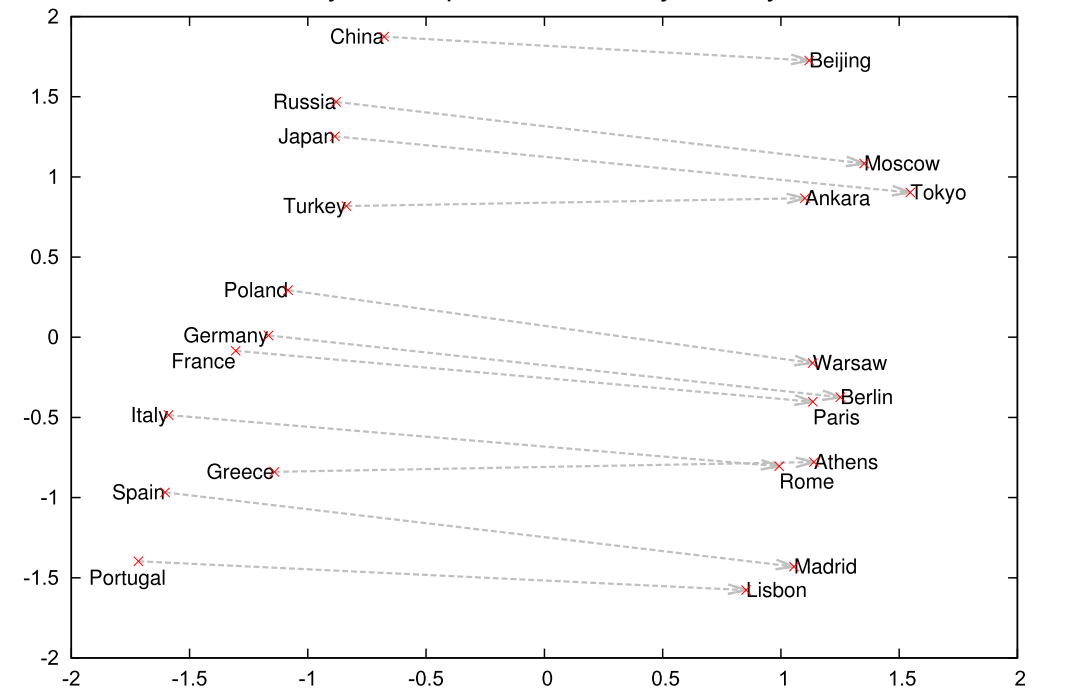
\includegraphics[height=7cm,width=\linewidth]{Figures/fig_word_vec_contries_capitals.png}
 \centering
 \caption{Two dimensional projection of Skip-gram vectors of countries and their capitals. Image extracted from the original paper~\cite{DBLP:conf/nips/MikolovSCCD13}.}
 \label{fig:countries_capitals}
\end{figure*} 
In Figure~\ref{fig:countries_capitals} Skip-gram model is capable of grouping concepts and reflects the implicit relationship, between the words. For example, the distance between countries and capital cities is approximately same or the calculation of vec("Madrid") - vec("Spain") + vec("France") is closer to vec(“Paris”) than to any other word vector~\cite{}. %here there was something  
In addition, the word vectors from the embedding models can be leveraged to construct document vectors. The generated word and/or document vectors then can be utilized in wide range of NLP tasks such as document classification, question answering, sentiment analysis, etc. 

Beside word embedding models, \textit{document embedding} models are proposed to generate the distributed representation of texts, i.e., documents, paragraphs, sentences. The basic idea of these models is that utilizing context word of documents to construct document vectors. \\
In the following, we give an overview of the most prominent word and document embedding models: \\
\begin{itemize}
\item \textbf{PTE~\cite{PTE}.} PTE aims to learn distributed representation of text in a semi-supervised fashion. In other words, PTE leverages both labeled and unlabeled data to learn the representation of documents. Further, unlike other embedding models such as Skip-gram which do not use any labeled data and generalizable for a variety of tasks, PTE designed to be utilized from a particular task.  More precisely, the vector representations can be easily fine tuned for a certain task with a set of labeled dataset. The general workflow of PTE is shown in Figure~\ref{fig:PTE}.
\begin{figure*}[h]
 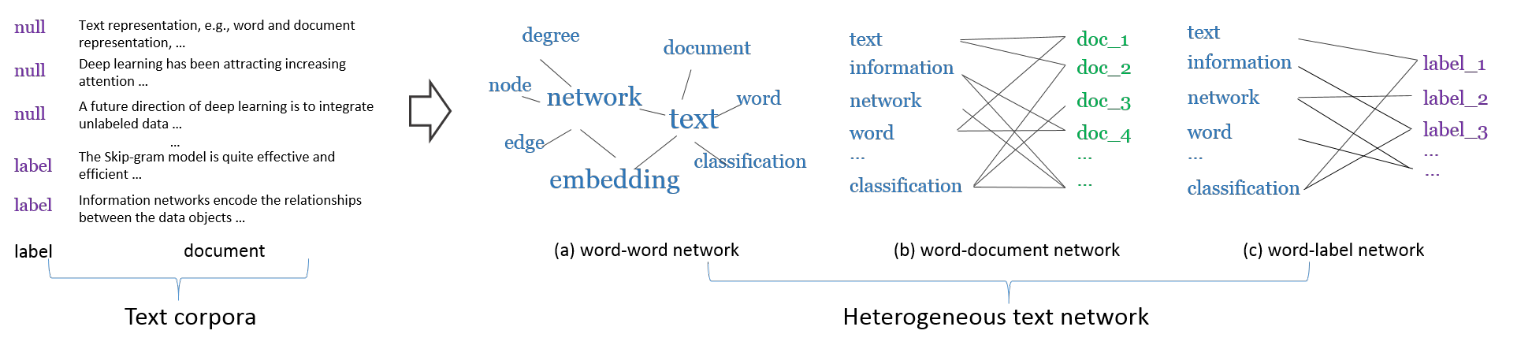
\includegraphics[width=\linewidth]{Figures/fig_PTE.png}
 \caption{Overview of converting text corpora to heterogeneous text network. Image extracted from the original paper~\cite{PTE}.}
 \label{fig:PTE}
\end{figure*} 
Given a large text corpora PTE first encodes the different co-occurrence information of between words-words, words-documents and words-labels. 
Word-word network (see Figure~\ref{fig:PTE}a) captures the co-occurrence of words in the same local context. The weight of the each edge of the network determined by the number of times that two word co-occur in the context windows. Word-document network (see Figure~\ref{fig:PTE}b) encodes the co-occurrence information of words in documents. The weight of an edges between a word and document defined by the number of times the word appears in the document. Word-label network captures the information of category level word co-occurrences. The weight between the word $w_{i}$ and category word $c_{j}$ is $w_{ij}$ which is defined as: $w_{ij} = \sum_{(d:l_{d}=j)} {n_{di}}$ where $l{d}$ is a class label of document $d$ and $n_{di}$ is term frequency of word $v_{i}$. Finally, the combination of word-word, word-document, and word-label networks constitutes the heterogeneous text network. Such network is being exploited by PTE to learn the latent representation of words while preserving the second order proximity (see Section~\ref{subsec:network_embedding_models}).

The overall heterogeneous network consists of three homogeneous networks, i.e., the word-word, word-document and word-label networks. PTE~\cite{PTE}, to embed each of these networks, aims to capture the second order proximity~\cite{tang2015line}.
To model the second-order proximity of a homogeneous network, for each edge $(v_i,v_j)$, the conditional probability $p(v_{j}|v_{i})$ is defined as follows~\cite{tang2015line}: 
\begin{equation}
%p(v_{j}|v_{i})=\frac{exp(-\vec{u}_{j}^{T}\cdot\vec{u}_{i})}{\sum\limits_{k=1}^{|V|} exp(-\vec{u}_{k}^{T}\cdot\vec{u}_{i})}\,,
p(v_{j}|v_{i})=\frac{exp(-\vec{u}_{j}^{T}\cdot\vec{u}_{i})}{\sum\limits_{v_k\in V} exp(-\vec{u}_{k}^{T}\cdot\vec{u}_{i})}\,,
%\raisepunct{,}
%p_{1}(v_{j}|v_{i})=\frac{exp(-\vec{u}_{i}^{T}.\vec{u}_{j})}{\sum_{k=1}^{V}exp(-\vec{u}_{i}^{T}.\vec{u}_{j})}
\end{equation}
where $V$ is the set of vertices connected with $v_i$ in the network, $\vec{u}_{i}$, $\vec{u}_{j}$ and $\vec{u}_{k}$ are the vectors of vertices $v_i$, $v_j$ and $v_k$, respectively. The empirical probability of $p(v_{j}|v_{i})$ can be defined as $\hat{p}(v_j|v_i)=\frac{w_{ij}}{d_i}$, where $d_i$ is the out-degree of $v_i$ and $w_{ij}$ is the weight of the edge $(v_i,v_j)$.

In order to preserve the second-order proximity, the conditional distribution $p(v_{j}|v_{i})$ is made close to $\hat{p}(v_{j}|v_{i})$ based on the KL-divergence over the entire set of vertices in the network, such that the model minimizes the following objective function:
\begin{equation}\label{optimizationHomo}
O=-\sum_{(v_i,v_j) \in E}w_{ij} \textrm{log} \,(p(v_{j}|v_{i}))\,,
\end{equation}

The embedding of the individual word-word, word-document and word-label networks are learned simultaneously by minimizing the following objective function:
% $O={O}_{ee}+{O}_{ec}$ .
 \begin{equation}\label{optimizationHet}
 O_{pte}={O}_{ww}+{O}_{wd}+{O}_{wl}\,,
 \end{equation}

where ${O}_{ww}$, ${O}_{wd}$ and ${O}_{wl}$ are the objective functions defined in Eq.~(\ref{optimizationHomo}) for the homogeneous word-word, word-document and word-label networks, respectively. 
To optimize the objective function in Eq.~(\ref{optimizationHet}), the edges are firstly collected from these three homogeneous networks as three sets, one for word-word edges, one for word-document edges and the other for word-label edges, and then in each training iteration, edges are sampled from each set to update the model. Readers can refer to~\cite{PTE,LINE}, for the detailed optimization process.

Once the word vectors are learned then the  representation of an arbitrary piece of text i.e., words $w_1, w_2, w_3,..., w_n$ present in text $d$ is simply inferred as the average of the word representations as follows:

\begin{equation}
\vec d= \frac{1}{n}\sum_{i=1}^{n}\vec u_{i}.
\end{equation}

\item \textbf{Skip-gram~\cite{DBLP:journals/corr/abs-1301-3781}.} Skip-gram model learns the low dimensional representation of words while capturing syntactic and semantic word relationships from a given large corpus. The word vectors are computed leveraging 2-layer simple feed forward neural networks. Training Skip-gram is very efficient, i.e., depending on the size of the corpus and the parameters it can only take couple of hours. Moreover, the model can be easily adapted to domain specific applications, e.g., patent classification by training it with a relevant large text corpus.
The Figure~\ref{fig:skip_gram} depicts the overview of Skip-gram model. 
\begin{figure*}[h]
\centering
 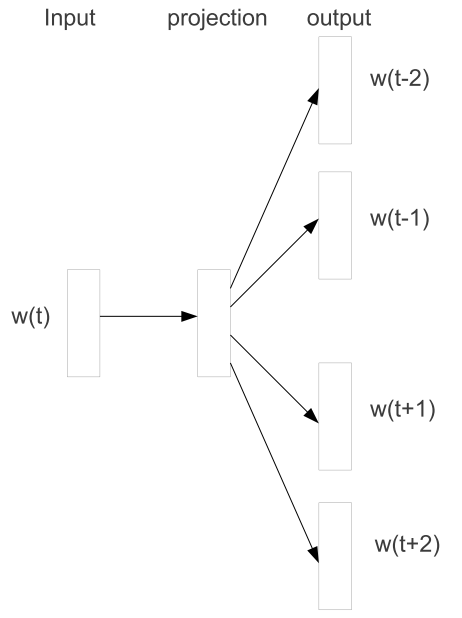
\includegraphics[height=4cm,width=4cm]{Figures/fig_skip_gram.png}
 \caption{Overview of Skip-gram model architecture. Image extracted from the original paper~\cite{DBLP:journals/corr/abs-1301-3781}.}
 \label{fig:skip_gram}
\end{figure*} \\
The basic idea of the model is to given a word  $w(t)$ from a sentence, the model tries to predict the  probability for every word in the vocabulary of being the \textit{nearby word}, i.e., window of surrounding context words. According to Figure~\ref{fig:skip_gram}, surrounding context words of $w(t)$ are $w(t-2), w(t-1), w(t+1), w(t+2)$. Note that the size of the window is an input parameter. %Ideally, the actual nearby words should have the higher probability than the other 

The objective of the training Skip-gram model is to compute word vectors that are useful for predicting the surrounding words in a text. Then the objective of Skip-gram model is to maximize average log probability a given sequence of words $w_1, w_2, w_3, ..., w_T$ as follows: 

\begin{equation}
\frac{1}{T}\sum_{t=1}^{T}\sum_{-c \leq j\leq c, j\neq0 } \textrm{log} p(w_{t+1}|w_{t})
\end{equation}
where $c$ is the size of the training context and specified with the window size. The higher the window size more the training samples are. \\
The probability $p(w_{t+1}|w_{t})$ defined by using softmax function: 
\begin{equation}
p(w_{O}|w_{I})=\frac{exp({v^{'}_{w_O}}^{T} {v}_{w_{I}})}{\sum\limits_{w=1}^{W} exp({v^{'}_w}^{T} {v}_{w_{I}})}
\end{equation}
where $v_w$ and $v'_w$ are input and output vector representation of $w$, and $W$ in the number of entire words in the vocabulary. Computing such an equation for each training sample is a very expensive task. Therefore, instead of calculating full softmax, hierarchical softmax which is computationally much more efficient is being used. Unlike softmax which evaluates $|W|$ output nodes to find the probability distribution, hierarchical softmax evaluates only approximately $\textrm{log}_2(W)$ nodes. The output layer is represented as a binary tree in Hierarchical softmax. Each leaf node corresponds to a word $w$, $w \in W$. For each node the tree relatively represent the probability of its child node(s). The hierarchical softmax defined as follows:

\begin{equation}
\displaystyle P(w|w_I) \prod_{j=1}^{L(w)-1} \sigma([n(w,j+1)=ch(n(w,j))]\cdot {v^{'}_{n(w,j)}}^{T} {v}_{w_{I}} )  
\end{equation}
where $n(w,j)$ is $j$-th node on the path from the root to $w$, $L(w)$ is the length of this path and $\sigma(x)=1/(1+exp(-x))$. Given the equation of hierarchical softmax the cost of computing $P(w|w_I)$ is on average not greater than $\textrm{log}W$.

Furthermore, the authors simply Noise Contrastive Estimation (NCE)~\cite{cite} method as alternative to the hierarchical softmax. NCE is based on the idea that a successful should be capable of differentiation data from the noise with the help of logistic regression model. Then for the Skip-gram model  the goal is to given a $P(w_O|w_I)$ distinguish between the target word $w_O$ and the negative samples which are drawn randomly. For each data sample there are $k$ negative samples. Then the objective of Negative sampling defined as follows: 
\begin{equation}
 \textrm{log}\sigma({v^{'}_{w_O}}^{T} {v}_{w_{I}} )+ \sum_{i=1 }\mathbb{E}_{w_i\sim P_n(w)}\left[ \textrm{log}\sigma({- v^{'}_{w_O}}^{T} {v}_{w_{I}} ) \right] 
\end{equation}
where $P_n(w)$ is noise distribution from which the negative samples are drawn. $P_n(w)$ is a parameter which authors show that the uniform distribution performs the best for several tasks.

The Skip-gram models requires large corpora for learning the vector representation of words and the frequency of words has impact on the quality of the vectors. In very large corpora, usually the most frequent are the least informative words (e.g., "the", "a", "an", "up"). To address this problem a simple subsampling approach has been defined as:
\begin{equation}
P(w_i)=1-\sqrt{\frac{t}{f(w_i)} }
\end{equation}
where $f(w_i)$ is the frequency of word $w_i$ and $t$ is a chosen threshold, around $10^{-5}$. 

Overall, the Skip-gram model has been the base of many embedding models such as DeepWalk, node2vec, doc2vec etc. In addition, it is still one of the most standard baselines for many word, document and network embedding models.\\\todo{here you can explain word2vec model in 2 variations, i.e, skip-gram and cbow.}
% two-layer neural networks
%look at the words nearby and pick one at random. The network is going to tell us the probability for every word in our vocabulary of being the “nearby word” that we chose.

% and CBOW
\begin{figure*}[t]
\centering
 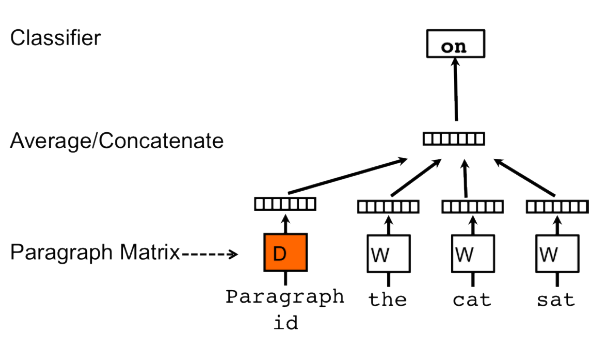
\includegraphics[height=5cm,width=8cm]{Figures/fig_doc2vec.png}
 \caption{Overview of doc2vec model architecture. Image extracted from the original paper~\cite{DBLP:conf/icml/LeM14}.}
 \label{fig:doc2vec}
\end{figure*} 
\item \textbf{Doc2vec~\cite{DBLP:conf/icml/LeM14}.}
Doc2vec model extends Skip-gram model in order to obtain latent representation of texts  i.e., sentences, paragraphs, documents. Unlike Skip-gram which learns only the vector representation of words from large corpora, doc2vec learns vector representation of words as well as the documents (in which the words present).  Doc2Vec is an unsupervised algorithm which is trained to to be useful for predicting the words in documents to learn the document representations. Therefore, semantically similar documents or documents that share many common words expected to be located close to each other in the common vector space. 
The Figure~\ref{fig:doc2vec} illustrates the overview of doc2vec architecture. The document vector $D$ is concatenated (or averaged) with the word vectors $W$ from the document, then the model predicts the following word in the given context.

The model is inspired by the Skip-gram architecture, which is trained to predict a word given context words. The doc2vec models is also trained to predict next word from given context information. However, in doc2vec the input is not only words but also a document vector which is treated similar to the word vectors. Every word and every document from the given corpora mapped to unique vector. After the training word as well as document vectors can be used in wide range of NLP task such as text classification, question answering, text summarization etc. Since the architecture of doc2vec is very similar to Skip-gram, we do not discuss the technical details here. \\   

%\item \textbf{ELMo.}\\
\item \textbf{BERT~\cite{DBLP:conf/naacl/DevlinCLT19}.} Bidirectional Encoder Representations from Transformers (BERT) is a language representation model which utilizes both jointly right and left context in all layers to pretrain deep bidirectional representations. The pretrained model then can be easily fine tuned to create language representation model for wide range natural language processing tasks. The technical implementation of BERT almost identical to the previous study by .... therefore, here we skip the technical details of the model.
The framework of BERT is shown in Figure~\ref{fig:bert}.
\begin{figure*}[h]
\centering
 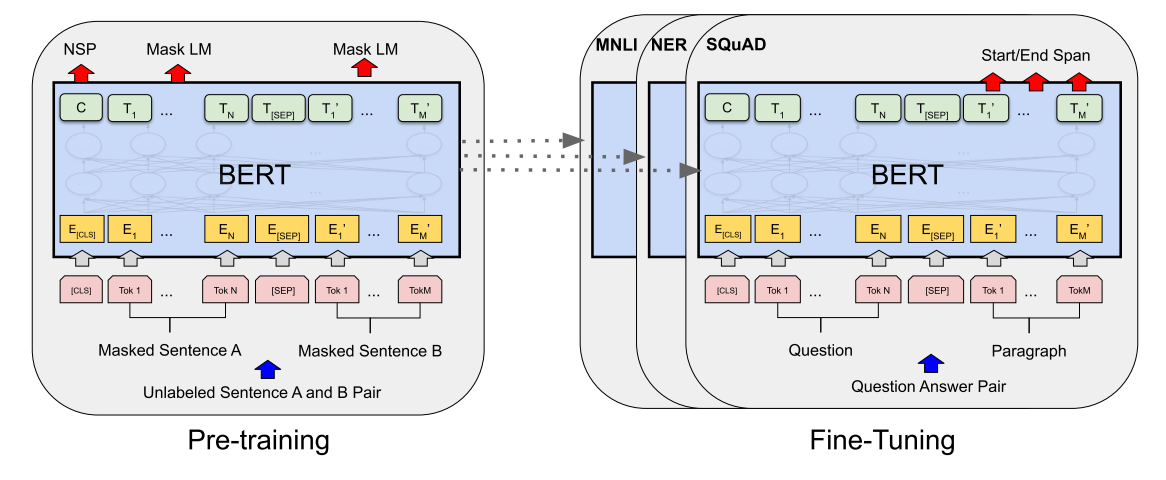
\includegraphics[width=\linewidth]{Figures/fig_BERT.png}
 \caption{Overview of BERT architecture. Image extracted from the original paper~\cite{DBLP:conf/naacl/DevlinCLT19}.}
 \label{fig:bert}
\end{figure*} 

BERT framework consists of two main steps (see Figure~\ref{fig:bert}) namely, pre-training and fine-tuning. Input to BERT is sequence of words which can be a single sentence or a pair of sentences. The first token of every input is always a special token ([CLS]) and the pair of sentences are separated by another special token ([SEP]). The input embedding of each token denoted as $E$ and the final hidden vector for the $i^{th}$ input token as $T_i$. \\
During the pre-training phase which is illustrated left part of Figure~\ref{fig:bert}, model is trained with two unsupervised tasks, namely, masked language modeling and next sentence prediction.
Masked language model task randomly masks some tokens of the input, then predicts those masked tokens. In this task, the final hidden vectors of masked tokens are fed into an output softmax over the vocabulary. Overall, the model tries to predict the masked inputs instead of an entire input.\\
The second task of pre-training is binarized next sentence prediction (NSP). The goal of the task is to train the model to learn the relationship between two sentences. In order to train the model, the dataset generation phrase is straightforward. Given a sentence A and if the sentence B is the actual next sentence that follows A then labelled as IsNext and the randomly selected sentences from the corpus would be labeled as NotNext. As shown in Figure~\ref{fig:bert}, $C$ which is the final hidden vector of the special token ([CLS]) is used for next sentence prediction task.\\
The second component of the frame work is fine-tuning as shown in Figure~\ref{fig:bert} (right). After the pre-training phase, all the parameters of the model can be fine-tuned with labeled data. In other words, depending on the application at hand such as question answering task, inputs and outputs, i.e., question-passage pairs are plugged into BERT in order to fine tune all the parameters. Note that  for each application at hand there are different fine-tuned models. 


\end{itemize}

%PTE
%CBOW, Skip-Gram
%ELMo , GPT , BERT
%doc2vec
%
\subsection{Network Embedding Models}
\label{subsec:network_embedding_models}
Networks are powerful structures for modeling many sophisticated systems such as information networks, social networks, etc. To be able to process the network data for variety of tasks such link prediction, node classification, node clustering etc. effective and efficient representation of the network data is crucial. The traditional explicit network representation methds such as adjency matrixes\todo{check} seem to be quite inefficient in large-scale networks. Motivated by this challenge several network emdedding models have been proposed~\cite{}.
Network embedding models are designed to generate the low dimensional vector representation of nodes based on the assumption that the structure of the network should be reflected in the learned feature representations. The relation of the nodes in the network, i.e., the connection between the nodes preserved also in the vector space as well. In other words, nodes that are considered to be similar based on the structure of the network should be placed closely in the vector space where similarity is measured by the distance between the nodes. 
Figure~\ref{karate} illustrates an example of an embedding model. Given the input karate network (Figure~\ref{}b) the similar nodes (that share the same color) placed close to each other in the embedding space (Figure~\ref{}b). The network embedding model aims to preserve the network structure while learning the dense and continuous representations of nodes in a low dimensional space. 
Traditionally, a network is represented as graph, hence following first we give the formal general definition of a Graph and then network embedding task.
\begin{definition}{(Graph):\\}
\textit{A $G(V, E)$ contains a set of vertices $V={}$ and set and a set of edges $E={}$ where E ⊆ (V × V).}
\end{definition}

\begin{definition}{(Network embedding):\\}
\textit{A network embedding function $f : V \rightarrow $ which maps each vertix $v \in V$ to  $d$ dimentional vector in Rd }
\end{definition}

There are two main goals that network embedding models aim to achieve in order to represent the nodes in a low dimensional space~\cite{survey}: (1) The original network can be reconstructed from the learned vector space, in other words, nodes that connected in the original network should be distance between them should be small. (2) The learned embedding space should be applicable to original network inference task such as identifying important nodes.

Moreover, to embed the nodes of a network into common vector space, different network embedding models adopt different approaches, i.e., matrix factorization, random walk, deep neural networks, etc. In this section we discuss the most commonly used approaches:  
\begin{itemize}
\item \textbf{Matrix Factorization.}\\
To represent a network topology matrices~\cite{survey} where each row and colom corresponds to a node are commonly used. Each entry in this matrix indicates the relation between the corresponding nodes. Network embedding models aim to find the low dimentional representation of nodes of the given network. Matrix factorization methids are common ways to achieve this purpose. Matrix factorization can be Given a matrix M  
%sepNE formula 1
\item \textbf{Random Walk.}\\
Random walks have been used in variety of applications such as .. as a similarity measure~\cite{deewalk}. In the context of network embeddings, random walk models are being exploited to generate random paths over a given network. By doing so, neighbourhood information of vertices can be extracted from the network. Network embedding models which exploit random walk techniques mainly relies on the neighbourhood information of vertices in order to generate vector representation of vertices. This idea highly relates to a neural language model by regarding a vertex as a word and a random walk is a sentence then the node neighborhood can be identified by co-occurence rate as in Skip-Gram model~\cite{survey}.   

\end{itemize}
Furthermore, deep neural networks are also commonly exploited by the several network embedding models~\cite{}\todo{find embedding models as an example}. Neural networks have been discussed in Section~\ref{secnn}.   


In the following we give the example of the most prominent network ebedding models applications:
\begin{itemize}
%cite each of them
\item \textbf{DeepWalk.}
DeepWalk network embedding model aims to learn distributed representation of the vertices in a given network by considering the neighborhood relations of vertices. To this end, the model attempts to conduct two main tasks; first, the model generates random walks on a given network and secondly, the representation of each vertex which is generated by the random walks (from the first step) is updated based on a neural language model. More precisely, DeepWalk relates the distribution of each vertex appearing in random walks to the distribution of words that appear in natural language~\cite{DBLP:journals/tkde/CuiWPZ19}. Motivated by this assumption, DeepWalk adapts a language model so called Skip-Gram to update the representation of each vertex generated by the random walks.
\begin{figure*}[h]
 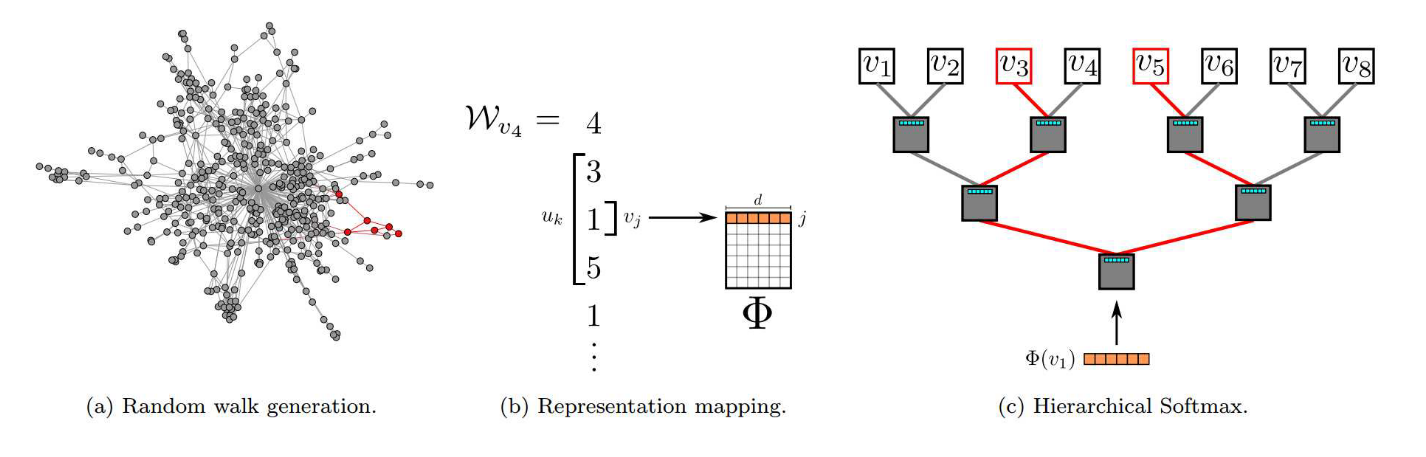
\includegraphics[width=\linewidth]{Figures/fig_deepwalk.png}
 \caption{Overview of DeepWalk. Image extracted from the original paper~\cite{}.}
 \label{fig:deepWalk}
\end{figure*} \\
Figure~\ref{fig:deepWalk} depicts the overview of the DeepWalk model. Given a graph the random walk generator (Figure~\ref{fig:deepWalk}a) randomly samples uniformly a vertex $v$ as a root of the random walk $W$. Then the walk uniformly samples the neighbour of the last visited vertex iteratively until the maximum length of the walk $t$ is reached. The maximum length of the walks ($t$) is an input parameter. Likewise, the number of walks at each vertex $\gamma$ is also an input parameter.\\ 
Skip gram model iterates over all collocation of vertices that appear within the given window size. In Section we have already \todo{Skip gram section, also check SkipGram vs Hsoftmax} introduced the Skip gram model, therefore, in this section we skip the technical details of it. As shown in Figure~\ref{fig:deepWalk}b each vertex $v$ is mapped to its current representation vector $\Phi(v)$. Finally, Hierarchical Softmax is used to learn the distributed representation of the vertices. \\
 
\item \textbf{LINE.}
Large-scale Information Network Embedding (LINE) learns latent representation of vertices of an arbitrary, i.e., undirected, directed, and/or weighted type of an information network. The model is capable of scaling to very large information networks. Moreover, LINE aims to optimize an objective function which preserves the local structure, i.e., \textit{first order proximity} and global structure, i.e., \textit{second order proximity} of a given network. 
\begin{figure*}[h]
\centering
 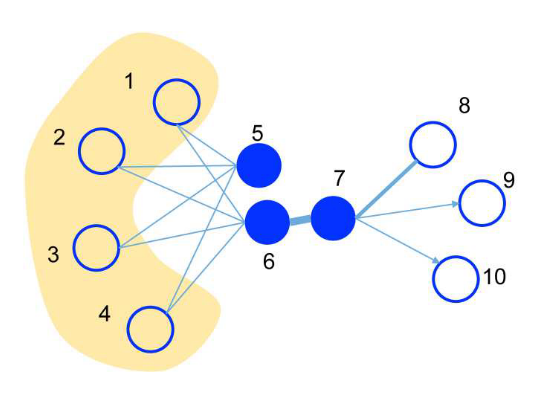
\includegraphics[height=5cm]{Figures/fig_LINE.png}
 \caption{An example of an information network. Image extracted from the original paper~\cite{LINE}.}
 \label{fig:LINE}
\end{figure*} \\
Figure~\ref{fig:LINE} illustrates an example of a simple information network. The thickness of the edges between vertices determines the strongness of the connections. 
First order proximity defined as the observed local pairwise proximity between two nodes~\cite{DBLP:journals/tkde/CuiWPZ19}. For example, in Figure~\ref{fig:LINE} the observed edge between vertex 6 and 7 is stronger, i.e., thicker. According the first order proximity vertex 6 and 7 should be placed closely in the vector space. On the other hand, the first order proximity between the vertex 5 and 6 is zero as there is no edge between them.
To model the first order proximity between vertices $v_i$ and $v_j$ the following joint probability defined as:
\begin{equation} \label{eq:jointProb}
p_{1}(v_{i},v_{j})=\frac{1}{1+exp(-\vec{u}_{i}^{T}\cdot\vec{u}_{j})}
\end{equation}
where $\vec{u}_{i}$ ($\vec{u}_{j}$) is the vector representation of node $v_i$ ($v_j$), respectively. In addition, its empirical probability can be defined as $\hat{p_1}(v_i,v_j)=\frac{w_{ij}}{W}$, where $W=\sum_{(i,j) \in E}w_{ij}$, $E$ is the set of edges between nodes in the network, and $w_{ij}$ is the weight of the edge $(i,j)$.
In order to preserve the first-order proximity, the model aims to minimize the KL-divergence between the two distributions $p_{1}(v_{i},v_{j})$ and $\hat{p_1}(v_i,v_j)$. By omitting some constants, the final goal is to minimize the following objective function:
\begin{equation}
O_{1}=-\sum_{(i,j) \in E}w_{ij} \textrm{log}p_{1}(v_{i},v_{j})
\end{equation}
Note that the first order proximity only applicable for the undirected graphs.

Second order proximity is determined between the two vertices through the shared neighborhood structures of the vertices. In other words, two nodes considered to be similar if they share the same neighbors according to the notation of second order proximity. For example, the vertex 5 and 6 in Figure~\ref{fig:LINE} should be placed closely as they share similar neighbors. 
To model the second-order proximity, for each edge $(i,j)$, the conditional probability is defined as follows: 
\begin{equation}
p_{2}(v_{j}|v_{i})=\frac{exp(-\vec{u}_{j}^{T}\cdot\vec{u}_{i})}{\sum\limits_{k=1}^{|V|} exp(-\vec{u}_{k}^{T}\cdot\vec{u}_{i})}
%p_{1}(v_{j}|v_{i})=\frac{exp(-\vec{u}_{i}^{T}.\vec{u}_{j})}{\sum_{k=1}^{V}exp(-\vec{u}_{i}^{T}.\vec{u}_{j})}
\end{equation}
where $V$ is the set of nodes connected with $v_i$ in the network. The empirical probability of $p_{2}(v_{j}|v_{i})$ can be defined as $\hat{p_2}(v_{j}|v_{i})=\frac{w_{ij}}{d_i}$, where $d_i$ is the out-degree of $v_i$. In order to preserve the second-order proximity, the conditional distribution $p_{2}(v_{j}|v_{i})$ is made close to $\hat{p_2}(v_{j}|v_{i})$ based on the KL-divergence over the entire set of nodes in the network, such that the model minimizes the following objective function:
\begin{equation}
O_{2}=-\sum_{(i,j) \in E}w_{ij} \textrm{log} p_{2}(v_{j}|v_{i})
\end{equation}

In order to keep both first-order and second-order proximities for each node, two LINE models are trained. Firstly, a LINE model is trained by preserving the first-order proximity, and then another LINE model is trained by preserving the second-order proximity. Finally, concatenating the embeddings of both models yields an embedding for each node. \\

\item \textbf{Node2vec.}
Scalable Feature Learning for Networks (node2vec) model is based on the idea of learning the latent representation of the vertices in a given network by maximizing the likelihood of preserving network neighborhoods of vertices. Node2vec extends a prior work, i.e., DeepWalk, which is based on rigid notions of network neighborhoods. Unlike DeepWalk, node2vec designs a biased random walk procedure which explores diverse neighborhoods.  In other words, node2vec leverages \nth{2} order random walk approach to generate neighbourhoods for vertices\todo{nodes or vertices}. The key contribution of the model is biased random walk strategy which is capable of exploring diverse neighbours of vertices.\\  
Given a network $G = (V, E)$ where $V$ is all the vertices and $E$ is all the edges between the vertices in the network. Let $f : V \to \mathbb{R}^d$ be the function that maps the each vertex to its corresponding distributed $d$ dimensional vector representation. For each source node (the start node of a random walk) $u\in V$ , $N_s(u) \subset V$ is defined as network neighborhood of $u$ generated by biased random walk strategy $S$.\\
$S$ generates biased random walks in order to sample the neighborhood nodes that smoothly interpolate between breadth-first sampling (BFS) and depth-first sampling (DFS). 
Then, given a source node $u$ and the length $l$ of the walk, $c_i$ the $i_{th}$ node in the walk generated by the following distribution:


\begin{equation}
    P(c_i = x| c_{i-1}=v )= \begin{cases}
    \frac{\pi_{vx} }{Z}, & \text{if $(v,x)\in E$}.\\
    0, & \text{otherwise}.
  \end{cases}
\end{equation}

where $c_0 =u$, $\pi_{vx}$ is the transition probability between nodes $v$ and $x$, and $Z$ is the normalization constant. \\
Assuming a random walk traversed edge $(t, v)$ and now resides at node $v$. For the next step, the walk evaluates the transition probabilities on edges $(v,x)$ leading from $v$. Then the transition probability $\pi_{vx}=\alpha_{pq}(t,x)\cdot w_{vx}$ can be set as follows:
\begin{equation}
    \alpha_{pq}(t,x)= \begin{cases}
    \frac{1}{p}, & \text{if $d_{tx}$=0}.\\
    1, & \text{if $d_{tx}$=1}.\\
    \frac{1}{q}, & \text{if $d_{tx}$=2}.\\
  \end{cases}
\end{equation}
where $d_{tx}$ denotes the shortest path distance between nodes $t$ and $x$. The parameter $p$ controls the likelihood of immediately revisiting a node in the walk whereas $q$ allows the search to differentiate between inward and outward nodes.%“inward” and “outward” nodes.

Finally, the model tries to optimize the following objective function as follows:
\begin{equation}\label{eq:node2vec_objective}
\max_{f} \sum_{u \in V } \textrm{log} Pr(N_S(u)|f_{u})
\end{equation}

which maximizes the log-probability of observing a network neighborhood $N_S(u)$ for a node $u$ conditioned on its feature representation, given by $f$.\\
In order to optimize the above objective function two assumptions are made as:
\begin{itemize}
\item The likelihood of observing a neighborhood node is independent of observing any other neighborhood node as:
\begin{equation}
 Pr(N_S(u)|f(u))= \prod_{n_i \in N_S(u)}Pr(n_i|f(u))
\end{equation}
\item A source node and neighborhood node have a symmetric effect over each other in feature space and this assumption modeled as follows:

\begin{equation}
P_{r}(n_{i}|f(u))=\frac{exp(f(n_i)\cdot f(u))}{\sum\limits_{v \in V} exp(f(v)\cdot f(u))}
%p_{1}(v_{j}|v_{i})=\frac{exp(-\vec{u}_{i}^{T}.\vec{u}_{j})}{\sum_{k=1}^{V}exp(-\vec{u}_{i}^{T}.\vec{u}_{j})}
\end{equation}

\end{itemize}
Finally with the two above assumptions the Equation~\ref{eq:node2vec_objective} simplifies as follows:
\begin{equation}\label{eq:node2vec_objective_final}
\max_{f} \sum_{u \in V }[ -\textrm{log}Z_u + \sum_{n_i \in N_S (u) }f(n_i) \cdot f(u)]
\end{equation}
where $Z_u$ is a per\_node partition function which is $Z_u= \sum\limits_{v \in V} exp(f(v)\cdot f(u))$. The partition function $Z_u$ is expensive to calculate especially for the large networks, therefore, similar to Skip-gram model negative sampling method is adapted to approximate $Z_u$ function and stochastic gradient ascent is used to optimize the Equation~\ref{eq:node2vec_objective_final}.\\

%As it can be seen from the objective function~\ref{Equation 1} of the model is an extension of 
%Skip gram model. However, the neighbourhood sampling method $S$  is the key contribution of the model which generates biased random walks in order to sample the neighborhood nodes that smoothly interpolate between breadth-first sampling (BFS) and depth-first sampling (DFS). 

\item \textbf{SepNE.}
Given a network SepNE model learns the latent representation of vertices in subsets and in separeta processes. By doing so the model avoids the effort to embed the nodes that are irrelevant to the application at hand. Therefore, the model is capable of scaling to very large networks.\\
\begin{figure*}[h]
\centering
 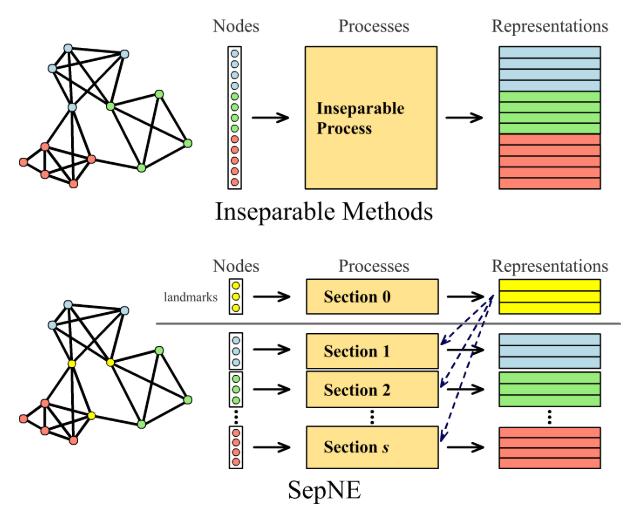
\includegraphics[height=5cm]{Figures/fig_SepNE.png}
 \caption{An example of Inseparable and separable network embedding processes. Image extracted from the original paper.}
 \label{fig:SepNE}
\end{figure*} \\
Figure~\cite{SepNE} depicts simple framework of SepNE and other models that do not separate the learning process. Traditional embedding models such as DeepWalk, LINE, node2Vec embed entire networks with inseparable processes. Unlike aforementioned models SepNE first, partitions the entire network into small subsets of nodes as shown in Figure~\ref{fig:SepNE}. A special set so called \textit{landmark set} which contains the highly interactive nodes in the network is constructed. The goal of the landmark set is to help for establishing references for different sets. First the landmark nodes are embedded, then the rest of the subsets are also embedded.\\
The model is formalized based on \textit{separated matrix factorization} (SMF). Let us firs briefly explain matrix factorization (MF) . Given a matrix $M$ which is of size $(nxn)$, matrix factorization aims to reduce $M$ into its constituent parts $W$ and $C$ that both $W$ and $C$ satisfy given constraints in Equation~\ref{mf} for reconstructing $M$. On the other, separated matrix factorization takes a network $G=(V,E)$ its proximity matrix $M$ and the partition setup $f : V $ .. as inputs. The goal of SMF is then to drive representations $(W_1, ..., W_s)$ and $(C_1, ..., C_s)$ for the partitioned sets that optimally reconstruct $M$ as: \\
\[M=\begin{pmatrix}
M_{11} &\cdots &M_{1s} \\
\vdots & \vdots & \ddots & \vdots\\
M_{s1} &\cdots &M_{ss}
\end{pmatrix}\]
where $M_{ij}$ indicates the proximities between $V_i$ and $V_j$.  In the training phase, in order order to achieve independence between subsets, each embedding section of every set utilizes only the proximities related to itself, e.g, embeddin section $V_i$ can only utilize $M_{i1}, M_{i2}, M_{i3},..., M_{is}$. \\
The SMF model that preserves only local information i.e., proximities within every set and ignores the intractions between the sets modeled as follows:
\begin{equation}\label{eq:node2vec_objective_final}
\min_{W_i, C_i} \Vert M_{ii} - W_{i}^T C_i\Vert , i=1,..., s.
\end{equation}

Moreover, landmark set (denoted as $V_0$) is also used as an additional information to derive the representation of the subsets. Landmark nodes established to indicate the proximities between subsets. The embedding method of the model for landmarks can be formulated as :
\begin{equation}
\min_{\Phi, \Psi} \Vert M_{00} - \Phi^T \Psi \Vert ,
\end{equation}
Then the representation of rest of the subsets are derived accordingly as:
\begin{equation}\label{eq:sepne_landmark_subets}
\min_{W_i, C_i} \left\Vert 
\begin{pmatrix}
M_{00}  &M_{0i} \\
M_{i0} &M_{ii}
\end{pmatrix} - 
\begin{pmatrix}
\Phi^T \Psi & \Phi^T C_{i} \\
W_{i}^T \Psi & W_{i}^T C_{i}
\end{pmatrix} \right\Vert , i=1,..., s.
\end{equation}
Equation~\ref{eq:sepne_landmark_subets} can be decomposed into local and landmark loss as: 
%formula 4 and 5

\begin{equation}
\mathcal{L}_{i}^{lc}(W,C)=\frac{1}{2}\Vert M_{ii} - W_{i}^T C_i\Vert_{F}^2 
\end{equation}

\begin{equation}
\mathcal{L}_{i}^{lc}(W,C)=\frac{1}{2}\Vert M_{0i} - \Phi^T C\Vert_{F}^2 +\frac{1}{2}\Vert M_{i0} - W^T \Psi\Vert_{F}^2 
\end{equation}

Assume as a first stage  the landmarks $(W_0 = \Phi, C_0 = \Psi)$ are embedded. Let $W_i, C_i \in \mathbb{R}^{(d\times|V_i|)}$ represented as linear combination as:

\begin{align*}
& W_i= \Phi A_i \\
& C_i= \Psi B_i, i=1,..., s
\end{align*}
where $A_i, B_i \in \mathbb{R}^{(d\times|V_i|)}$
To further combine global information to derive the latent representation of the embeddings a global loss function defined as follows:
\begin{equation}
\mathcal{L}_{i}^{gb}(A,B)=\frac{1}{2}(\Vert M_{i\bar{i}} - A^T M_{0\bar{i}}\Vert_{F}^2 +\Vert M_{\bar{i}i} - M_{\bar{i}0}B\Vert_{F}^2)
\end{equation} 

Then the final loss function which is combined $\lambda-$scaled global loss of SMF becomes:

\begin{align*}
& W_0= \Phi C_0= \Psi . \\
& W_i= \Phi A_i, C_i= \Psi B_i \\
& A_i,B_i=\underset{A,B}{\mathrm{argmin}}\mathcal{L}_{i}(A,B),  i=1,..., s. 
\end{align*}


\todo{Here we can add more emdedding models}

%\item \textbf{NetSMF.}

\end{itemize}
%DeepWalk, LINE, and node2vec


